\documentclass[class=minimal,border=0pt]{standalone}

\usepackage{tudfonts}

\usepackage{tikz}
\usetikzlibrary{calc}
\usetikzlibrary{matrix}
\usetikzlibrary{positioning}

\begin{document}

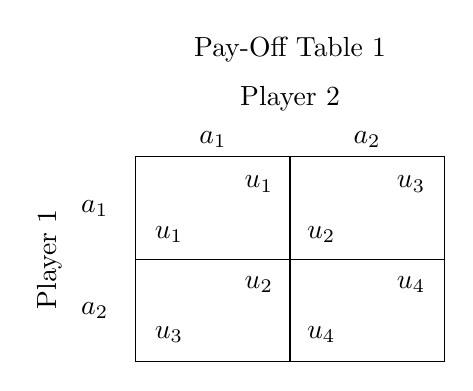
\begin{tikzpicture}

\matrix[matrix of math nodes,every odd row/.style={align=right},every even row/.style={align=left},every node/.style={text width=1.5cm},row sep=0.2cm,column sep=0.2cm] (m) {
$u_{1}$&$u_{3}$\\
$u_{1}$&$u_{2}$\\
$u_{2}$&$u_{4}$\\
$u_{3}$&$u_{4}$\\
};
\draw (m.north east) rectangle (m.south west);
\draw (m.north) -- (m.south);
\draw (m.east) -- (m.west);

\coordinate (a) at ($(m.north west)!0.25!(m.north east)$);
\coordinate (b) at ($(m.north west)!0.75!(m.north east)$);
\node[above=5pt of a,anchor=base] {$a_{1}$};
\node[above=5pt of b,anchor=base] {$a_{2}$};

\coordinate (c) at ($(m.north west)!0.25!(m.south west)$);
\coordinate (d) at ($(m.north west)!0.75!(m.south west)$);
\node[left=2pt of c,text width=.5cm]  {$a_{1}$};
\node[left=2pt of d,text width=.5cm]  {$a_{2}$};

\node[above=13pt of m.north] (firm b) {Player 2};
\node[left=1.1cm of m.west,rotate=90,align=center,anchor=center] {Player 1};

\node[above=2pt of firm b]  {Pay-Off Table 1};
\end{tikzpicture}

\end{document}